% !TEX root =../ECE343_Slides_Rogers.tex
\def\lessonNum{2}

%\begin{comment}
\section{Schedule}
\renewcommand{\arraystretch}{1}
\begin{frame}{}
	\begin{textblock}{14}(0.5,1.75)
	\def\myfontsize{footnotesize}
	
\setcounter{mylnum}{1}
\begin{center}
\begin{\myfontsize}
\begin{tabular}{| c | l | c | l |}
\hline
\textbf{Lesson} 		  	& \textbf{Topics}             & \pbox{5cm}{\textbf{Reading}}	& \textbf{Notes}		\\ \hline\hline
\ifnum\lessonNum=\value{mylnum} \rowcolor{green!20!white}\fi
	\themylnum  
	& Course Overview  \& Introduction		
	& Ch.1 
	&  LO 1.1-1.2 
	\stepcounter{mylnum}\\ \hline \hline
\rowcolor{gray!20!white}\multicolumn{4}{| c |}{\textbf{Chapter 2: Electric and Magnetic Fields}}	\\ \hline\hline
\ifnum\lessonNum=\value{mylnum} \rowcolor{green!20!white}\fi
	\themylnum 	
	& Fields, Parameters, Field Quantities	
	& Ch. 2	
	& LO 2.1-2.2			
\stepcounter{mylnum}\\ \hline\hline
\rowcolor{gray!20!white}\multicolumn{4}{| c |}{\textbf{Chapter 3: Transmission Lines}}	 \\ \hline\hline	
\ifnum\lessonNum=\value{mylnum} \rowcolor{green!20!white}\fi
	\themylnum 	
	& Lumped Element Model				
	& 3.1-3.4 
	& LO 3.1		
\stepcounter{mylnum}\\ \hline
\ifnum\lessonNum=\value{mylnum} \rowcolor{green!20!white}\fi
	\themylnum 	
	& Telegrapher's Equations
	& 3.5-3.6
	&  LO 3.1	
\stepcounter{mylnum}\\ \hline
\ifnum\lessonNum=\value{mylnum} \rowcolor{green!20!white}\fi
	\themylnum 	
	&  Characteristic Impedance \& Wave Propagation	
	& 3.7-3.9		
	& LO 3.2						
\stepcounter{mylnum}\\ \hline
\ifnum\lessonNum=\value{mylnum} \rowcolor{green!20!white}\fi
	\themylnum 	
	& Coaxial,  Reflection Coefficient, VSWR	
	& 3.10,3.12-3.14	
	& LO 3.2-3.3		
\stepcounter{mylnum}\\ \hline 
\ifnum\lessonNum=\value{mylnum} \rowcolor{green!20!white}\fi
	\themylnum 	
	&  Terminated Transmission Lines	
	&  3.15,3.17-3.19
	& LO 3.4		
\stepcounter{mylnum}\\ \hline 
\ifnum\lessonNum=\value{mylnum} \rowcolor{green!20!white}\fi
	\themylnum	
	& Impedance Matching	
	& 3.21-3.23
	& LO 3.4 			
\stepcounter{mylnum}\\ \hline 
\ifnum\lessonNum=\value{mylnum} \rowcolor{green!20!white}\fi
	\themylnum  
	& Impedance Matching	
	& 3.21-3.23
	& LO 3.4		
\stepcounter{mylnum}\\ \hline 
\ifnum\lessonNum=\value{mylnum} \rowcolor{green!20!white}\fi
	\themylnum	
	& Smith Charts
	& Supplemental
	& LO 3.5
\stepcounter{mylnum}\\ \hline 
\ifnum\lessonNum=\value{mylnum} \rowcolor{green!20!white}\fi
	\themylnum	
	& Smith Charts
	& Supplemental 
	& LO 3.5					
\stepcounter{mylnum}\\ \hline 
\ifnum\lessonNum=\value{mylnum} \rowcolor{green!20!white}\fi
	\themylnum	
	& Smith Charts
	& Supplemental 
	& LO 3.5	
\stepcounter{mylnum}\\ \hline 
\ifnum\lessonNum=\value{mylnum} \rowcolor{green!20!white}\fi
	\themylnum	
	& Smith Charts
	& Supplemental 
	& LO 3.5	
\stepcounter{mylnum}\\ \hline 

\ifnum\lessonNum=\value{mylnum} \rowcolor{green!20!white}\fi
	\themylnum	
	& Transients		
	& Supplemental 
	& LO 3.6	 
\stepcounter{mylnum}\\ \hline \hline
\ifnum\lessonNum=\value{mylnum} \rowcolor{green!20!white}\fi
	\themylnum 	
	& Flex Day
	& 
	& 	
\stepcounter{mylnum}\\ \hline 
\ifnum\lessonNum=\value{mylnum} \rowcolor{green!20!white}\fi
	\themylnum 	
	& Reflection/Transmission Coefficient Lab
	& Lab Packet
	& LO 3.7		
\stepcounter{mylnum}\\ \hline 
\ifnum\lessonNum=\value{mylnum} \rowcolor{green!20!white}\fi
	\themylnum 	
	& Reflection/Transmission Coefficient Lab
	& Lab Packet
	& LO 3.7		
\stepcounter{mylnum}\\ \hline 
\rowcolor{gray!20!white}\multicolumn{4}{| c |}{\textbf{Chapter 4: Vector Analysis}} \\ \hline\hline
\ifnum\lessonNum=\value{mylnum} \rowcolor{green!20!white}\fi
	\themylnum	
	& Vector \& Coordinate System Review
	& Ch. 4
	&LO 4.1-4.4 \textbf{GR 1 due}	
\stepcounter{mylnum}\\ \hline 
\rowcolor{gray!20!white}\multicolumn{4}{| c |}{\textbf{Chapter 5: Electrostatics}}\\ \hline\hline
\ifnum\lessonNum=\value{mylnum} \rowcolor{green!20!white}\fi
	\themylnum	
	& Coulomb's Law
	& 5.1-5.3
	& LO 5.1
\stepcounter{mylnum}\\ \hline 
\ifnum\lessonNum=\value{mylnum} \rowcolor{green!20!white}\fi
	\themylnum	
	& Surface and Volume Charge			
	& 5.4
	& LO 5.1
\stepcounter{mylnum}\\ \hline 
\ifnum\lessonNum=\value{mylnum} \rowcolor{green!20!white}\fi
	\themylnum	
	& Gauss' Law (Integral Form)
	& 5.5-5.6
	& LO 5.2		 					
\stepcounter{mylnum}\\ \hline 
\ifnum\lessonNum=\value{mylnum} \rowcolor{green!20!white}\fi
	\themylnum	
	& Gauss' Law (Differential Form)		
	& 5.7-5.8
	& LO 5.2	 	
\stepcounter{mylnum}\\ \hline 
\ifnum\lessonNum=\value{mylnum} \rowcolor{green!20!white}\fi
	\themylnum	
	& Electric Potential	
	& 5.9-5.10, 5.15
	&  LO 5.3	
\stepcounter{mylnum}\\ \hline 
% <---- line 129 should be 20 lessons, based on 6 lines per lesson, starting at line 9 
\end{tabular}			
\end{\myfontsize}
\end{center}

	\end{textblock}
\end{frame}

%%%%%%%%%%%%%%%%%%%%%%%%%%%%%%%%%%%%%%%%%%%%%%%%%%%%%
%%%%%%%%%%%%%%%%%%%%%%%%%%%%%%%%%%%%%%%%%%%%%%%%%%%%%
\section{LO's}

\begin{frame}{Ch 2 Learning Objectives}
	\begin{textblock}{14}(0.5,5)
	\begin{myblock}[0.9]{}
		\begin{enumerate}[{2}.1]
			\setlength{\itemsep}{18pt}
			\item \alert{I can recall the definition of scalar fields, vector fields, phasors, and Euler's identity.}
			\item \alert{I can explain the basic terms and quantities used to describe electromagnetic fields.}
		\end{enumerate}
	\end{myblock}
	\end{textblock}
\end{frame}


%%%%%%%%%%%%%%%%%%%%%%%%%%%%%%%%%%%%%%%%%%%%%%%%%%%%%
%%%%%%%%%%%%%%%%%%%%%%%%%%%%%%%%%%%%%%%%%%%%%%%%%%%%%

\begin{frame}{What is a field?}
	\begin{textblock}{14.5}(0.5,2)

		\begin{myblock}[0.9]{Field - Definition}	
			
			A field is the continuum of values of a quantity as a function of position and time. 
			
			\vspace{12pt}
			
			Fields can be \handoutgap{1in}{Scalar} or \handoutgap{1in}{Vector}
				
		\end{myblock}
	\end{textblock}
	\begin{textblock}{8}(0.5,7)

		\begin{myblock}[0.9]{Scalar Examples}	
			
			\vspace{1in}
				
		\end{myblock}
	\end{textblock}
	\begin{textblock}{8}(8,7)
		\begin{myblock}[0.9]{Vector Examples}	
			
			\vspace{1in}
				
		\end{myblock}

	

	\end{textblock}

%	\begin{textblock}{7.5}(0.5,8.5)
%	\scalebox{0.65}{
%	\begin{tikzpicture}
%	 
%		 \begin{axis}[small,view={0}{90}, colorbar, domain=-100:100, domain y = -100:100] 
%			 \addplot3[surf,shader=interp,patch type=bilinear]{sin(5*sqrt(x^2 + y^2))};
%		\end{axis}
%	 
%	\end{tikzpicture}
%	 }
%
%\end{textblock}
% 
% 
%\begin{textblock}{7.5}(8,8.5)
%	\scalebox{0.65}{
%	\begin{tikzpicture}
%	\begin{axis}
%		\addplot3 [
%		    domain=-100:100,
%		    domain y = -100:100,
%		    samples = 50,
%		    samples y = 50,
%		    surf] {sin(5*sqrt(x^2 + y^2))};
%	\end{axis}
%	\end{tikzpicture}
%	}
%\end{textblock}
%	
\end{frame}

%%%%%%%%%%%%%%%%%%%%%%%%%%%%%%%%%%%%%%%%%%%%%%%%%%%%%
%%%%%%%%%%%%%%%%%%%%%%%%%%%%%%%%%%%%%%%%%%%%%%%%%%%%%

\begin{frame}{Field Representation}
\begin{textblock}{14.5}(0.5,5)

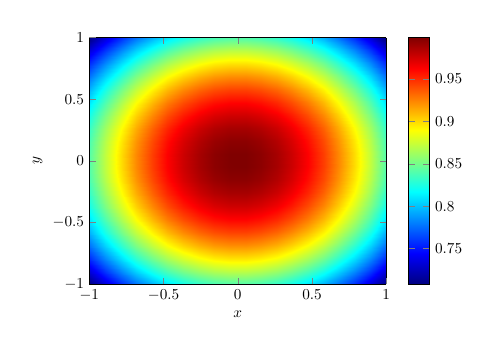
\begin{tikzpicture}[scale=0.55]
    \begin{axis}[
      view={0}{90}, % view angle
      xlabel=$x$,
      ylabel=$y$,
      zlabel=$z$,
      colormap/jet,
      colorbar,
      shader=interp,
      ]
      \addplot3[
        surf,
        domain=-1:1,   %radians
        domain y=-1:1, %radians
        samples = 20,
        title={$t=0$s}
        ]
      {sin(deg(x))/(x)*sin(deg(y))/(y)};
    \end{axis}
  \end{tikzpicture}%
  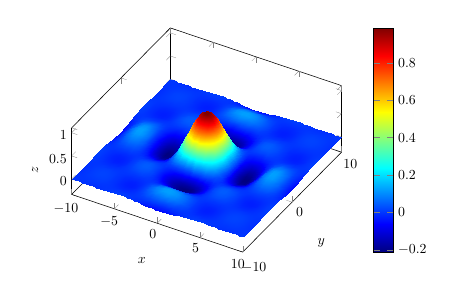
\begin{tikzpicture}[scale=0.5]
    \begin{axis}[
      view={30}{60}, % view angle
      xlabel=$x$,
      ylabel=$y$,
      zlabel=$z$,
      colormap/jet,
      colorbar,
      shader=interp,
      ]
      \addplot3[
        surf,
        domain=-10:10,
        domain y=-10:10,
        samples = 50,
        ]
      {sin(deg(x))/(x)*sin(deg(y))/(y)};
    \end{axis}
 \end{tikzpicture}
\end{textblock}

\end{frame}

%%%%%%%%%%%%%%%%%%%%%%%%%%%%%%%%%%%%%%%%%%%%%%%%%%%%%
%%%%%%%%%%%%%%%%%%%%%%%%%%%%%%%%%%%%%%%%%%%%%%%%%%%%%
\section{Electric}
\begin{frame}{Electric Field}
	\begin{textblock}{14.5}(0.5,2)
		\begin{myblock}[0.9]{Basics}
		\begin{itemize}
			\setlength\itemsep{12pt}
			\item \textbf{Electric Field Intensity} is a vector field that quantifies the \handoutgap{1in}{force} experienced by a charged particle due to the \handoutgap{1in}{influence} of a charge \handoutgap{1in}{not associated} with that particle. 
			
			\item \textbf{Units} $\longrightarrow$ \handoutgap{0.5in}{N/C} $\longrightarrow$ \handoutgap{0.5in}{V/m}
			
			\item \textbf{Direction} $\longrightarrow$ points in the direction in which \handoutgap{1in}{electric potential} is most rapidly decreasing. 
		\end{itemize}
		\end{myblock}

	
	\end{textblock}
	
	\begin{textblock}{8}(2,11)
		\begin{center}
		\begin{tikzpicture}[scale=1.5]
		\node[shade, shading=ball, circle, ball color=red, label={[yshift=-1cm, xshift=-0.5cm]\Large$+$} ] (pos) {};
		\node[right=2cm of pos, shade, shading=ball, circle, ball color=red, label={[yshift=-1cm, xshift=0.5cm]\Large$+$} ] (posright) {};
		\node[below right=0.05cm of pos, blue] {\scriptsize force};			
		\draw[line] (pos) -- (posright);
		\end{tikzpicture}%
		\vspace{1in}%
		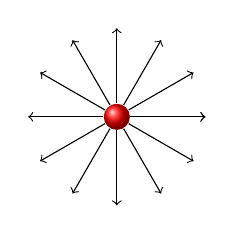
\begin{tikzpicture}[scale=1.5]
		\node[shade, shading=ball, circle, ball color=red ] (pos) {};
		\foreach \myangle in {0,30,60,...,360}{
				\draw[->] (pos) -- (\myangle:0.75cm);
			}
		\end{tikzpicture}
	\end{center}
	
	\end{textblock}
		
\end{frame}
%%%%%%%%%%%%%%%%%%%%%%%%%%%%%%%%%%%%%%%%%%%%%%%%%%%%%
%%%%%%%%%%%%%%%%%%%%%%%%%%%%%%%%%%%%%%%%%%%%%%%%%%%%%
%
\begin{frame}{Electromagnetic Material Properties}
		\begin{textblock}{14.5}(0.5,3)
			\begin{myblock}[0.9]{Permittivity, $\varepsilon$}
				Quantifies the effect of an electric field on a material. 
			\end{myblock}
			
			\begin{myblock}[0.9]{Permeability, $\mu$}
				Quantifies the effect of current in producing a magnetic flux density within a material.
			\end{myblock}

			\begin{myblock}[0.9]{Conductivity, $\sigma$}
				Quantifies the effect of current flow in response to an applied electric field. 
			\end{myblock}
		\end{textblock}
\end{frame}

%%%%%%%%%%%%%%%%%%%%%%%%%%%%%%%%%%%%%%%%%%%%%%%%%%%%%
%%%%%%%%%%%%%%%%%%%%%%%%%%%%%%%%%%%%%%%%%%%%%%%%%%%%%

\begin{frame}{Permittivity}
	\begin{textblock}{8}(0.5,5)
	\begin{itemize}
		\setlength\itemsep{32pt}
		\item Definition $\longrightarrow$ \handoutgap{0in}{the effect of material in determining the electric field in response to electric charge.}
		
		\item Physical Interpretation $\longrightarrow \vec{E} = \hat{r} \dfrac{q}{4\pi \varepsilon |r|^2}$
		
		\item Units $\longrightarrow$ \handoutgap{0in}{F/m}
	\end{itemize}
	\end{textblock}
	\begin{textblock}{8}(8.5,3)
	\scalebox{0.65}{
		\input{\mygraphicspath/ECE343/honeycomb_dim}
		}
	\end{textblock}
\end{frame}

%%%%%%%%%%%%%%%%%%%%%%%%%%%%%%%%%%%%%%%%%%%%%%%%%%%%%
%%%%%%%%%%%%%%%%%%%%%%%%%%%%%%%%%%%%%%%%%%%%%%%%%%%%%

\begin{frame}{Parallel Plate Capacitor}
	\begin{textblock}{14.5}(0.5,3)
		
		\begin{center}
			\includegraphics[scale=0.5]{ECE343/Parallel_Plate_Capacitor.jpg}
		\end{center}
		
	\end{textblock}
\end{frame}


%%%%%%%%%%%%%%%%%%%%%%%%%%%%%%%%%%%%%%%%%%%%%%%%%%%%%
%%%%%%%%%%%%%%%%%%%%%%%%%%%%%%%%%%%%%%%%%%%%%%%%%%%%%

\begin{frame}{Electric Flux Density}
	\begin{textblock}{14.5}(0.5,3)
	\scalebox{0.8}{
		\input{\mygraphicspath/ECE343/flux}
		}
	\end{textblock}
\end{frame}


%%%%%%%%%%%%%%%%%%%%%%%%%%%%%%%%%%%%%%%%%%%%%%%%%%%%%
%%%%%%%%%%%%%%%%%%%%%%%%%%%%%%%%%%%%%%%%%%%%%%%%%%%%%
\section{Magnetic}
\begin{frame}{Magnetic Fields}
		\begin{textblock}{8}(0.5,3)
			\includegraphics[scale=0.35]{ECE343/lorentz_force}
			\eq{
				\vec{F} = 
			}
		\end{textblock}
			
	\begin{textblock}{8.5}(6,2)
		\includegraphics[scale=0.4]{ECE343/electromagnet}
	\end{textblock}
\end{frame}

%%%%%%%%%%%%%%%%%%%%%%%%%%%%%%%%%%%%%%%%%%%%%%%%%%%%%
%%%%%%%%%%%%%%%%%%%%%%%%%%%%%%%%%%%%%%%%%%%%%%%%%%%%%

\begin{frame}{ Magnetic Fields, Permeability, Magnetic Flux Density}

		\begin{textblock}{14.5}(0.5,3)
		\begin{center}
		\begin{tikzpicture}[-]
		\def\my{1mm}
		
		%\draw [thick, red] (-2,-1) -- node [below] {} (2,-1) node (v3) {};
		%\draw [thick, red] (-2,1) -- node [above] {}  (2,1) ;
		
		\node[draw=blue, fill=white, rectangle, ,minimum size=1cm, inner sep=0, outer sep=0] (circ) at (0,0) {};
		%\draw [-{Latex},blue] (0,-1) -- (circ.south);
		\node [below] (v2) at (0,.5) {N};
		\node [above] (v1) at (0,-.5) {S};
		%\draw [-{Latex}, blue] (0,-.2) -- (0,.2) node [right] {$\vec p_{e}$};
		
		%\path[clip] (-2,0) -- (2,0) -- (2,2) -- (-2,2) -- cycle;
		\begin{scope}[scale=.3,on background layer]
		\clip[scale=3.3] (-3,-2) rectangle (3,2);
		\foreach \a [count=\b] in {1,2,3,4,5,6,7,8,9,10}{
		    \draw[domain=0:6.3,samples=500, line width=.1pt, decoration={markings,%
		        mark=at position 0.1 with {\arrowreversed{Stealth[width=\my,length=\my]}},
		        mark=at position 0.4 with {\arrow{Stealth[width=\my,length=\my]}},
		        mark=at position 0.5 with {\arrow{Stealth[width=\my,length=\my]}},
		        mark=at position 0.6 with {\arrow{Stealth[width=\my,length=\my]}},
		        mark=at position 0.9 with {\arrowreversed{Stealth[width=\my,length=\my]}},
		        mark=at position 1 with {\arrowreversed{Stealth[width=\my,length=\my]}},}, postaction=decorate] plot (xy polar cs:angle=\x r,radius={\a+\b*cos(2*\x r)});
		}
		\end{scope}
		\end{tikzpicture}
		\end{center}	
		
		\eq{
			\vec{B}(r) &= \mu \dfrac{q v}{4\pi R^2} \times \hat{R} \\[12pt]
			\vec{B} &= \mu\vec{H} 
		}
		
		\end{textblock}
\end{frame}


%%%%%%%%%%%%%%%%%%%%%%%%%%%%%%%%%%%%%%%%%%%%%%%%%%%%%
%%%%%%%%%%%%%%%%%%%%%%%%%%%%%%%%%%%%%%%%%%%%%%%%%%%%%
\section{Preliminary Concepts}
\begin{frame}{Electromagnetic Material Categories}
		\begin{textblock}{14.5}(0.5,3.5)
			\begin{itemize}
				\setlength\itemsep{18pt}
				\item \textbf{Homogeneous:} Material is the same, regardless of position of applied field. 

			
				\item \textbf{Isotroipc: } Material response is independent of orientation to the applied field. 
				
				\item \textbf{Linear: } Linear response to applied fields. 
			
				\item \textbf{Non-dispersive: } Material response is independent of frequency of applied field. 
			\end{itemize}
		\end{textblock}
\end{frame}

%%%%%%%%%%%%%%%%%%%%%%%%%%%%%%%%%%%%%%%%%%%%%%%%%%%%%
%%%%%%%%%%%%%%%%%%%%%%%%%%%%%%%%%%%%%%%%%%%%%%%%%%%%%

%\begin{frame}{Permeability, Magnetic Flux Density, Magnetic Field}
%	\begin{textblock}{4}(0.5,5.5)
%		\eq{
%			\vec{B}(r) &= \mu \dfrac{q v}{4\pi R^2} \times \hat{R} \\[12pt]
%			\vec{B} &= \mu\vec{H} 
%		}
%	\end{textblock}
%
%\end{frame}

%%%%%%%%%%%%%%%%%%%%%%%%%%%%%%%%%%%%%%%%%%%%%%%%%%%%%
%%%%%%%%%%%%%%%%%%%%%%%%%%%%%%%%%%%%%%%%%%%%%%%%%%%%%

%\begin{frame}{Preliminary Concepts - Fields}
%\begin{textblock}{14.5}(0.5,3)
%
%\begin{tikzpicture}
%    \begin{axis}[
%      view={30}{60}, % view angle
%      xlabel=$x$,
%      ylabel=$y$,
%      zlabel=$z$,
%      colormap/jet,
%      colorbar,
%      shader=interp,
%      ]
%      \addplot3[
%        surf,
%        domain=-10:10,
%        domain y=-10:10,
%        samples = 50,
%        ]
%      {sin(deg(x))/(x)*sin(deg(y))/(y)};
%    \end{axis}
% \end{tikzpicture}
%\end{textblock}
%
%\end{frame}




%%%%%%%%%%%%%%%%%%%%%%%%%%%%%%%%%%%%%%%%%%%%%%%%%%%%%
%%%%%%%%%%%%%%%%%%%%%%%%%%%%%%%%%%%%%%%%%%%%%%%%%%%%%
%%%%WAVES
% stuff for the wave graphics
\colorlet{xcol}{blue!70!black}
\colorlet{vcol}{green!60!black}
\colorlet{myred}{red!70!black}
\tikzstyle{vvec}=[->,vcol,very thick,line cap=round]
\tikzstyle{myarr}=[-{Latex[length=3,width=2]},myred]
\def\tick#1#2{\draw[thick] (#1) ++ (#2:0.1) --++ (#2-180:0.2)}
\def\xpeak#1{{(0.21+#1)*\xmax}}
\def\wave#1{
  \coordinate (F) at (\xpeak{#1},\ypeak);
  \draw[very thick,xcol]
    (-0.08*\xmax,0) -- ({(0.06+#1)*\xmax},0) to[out=0,in=180,looseness=0.5] (F)
    to[out=0,in=180,looseness=0.6]++ (0.25*\xmax,-\ypeak) -- (0.94*\xmax,0);
}

\begin{frame}[fragile]{Waves}
	\begin{textblock}{7}(0.5,3)
	\begin{myblock}[0.9]{Wave - Definition}	
		
		A wave is a time-varying field that continues to exist in the absence of the source that created it and is therefore able to transport energy.
			
	\end{myblock}
	\end{textblock}
	\begin{textblock}{8}(8.5,3)
	\only<1>{
		% WAVE t = 0
		\def\xmax{4.2}
		\def\ymax{2.0}
		\def\ypeak{0.80*\ymax}
		\def\v{0.17*\xmax}
		
		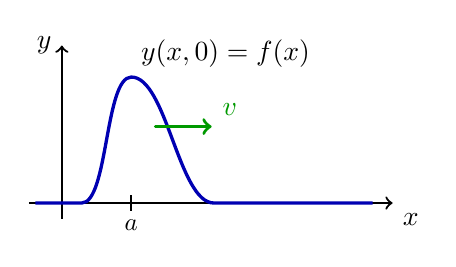
\begin{tikzpicture}
		  \draw[->,thick] (-0.1*\xmax,0) -- (\xmax,0) node[below right] {$x$};
		  \draw[->,thick] (0,-0.1*\ymax) -- (0,\ymax) node[left] {$y$};
		  \wave{0.0}
		  \node[above right] at (F) {$y(x,0)=f(x)$};
		  %\node[left] at (0.97*\xmax,0.65*\ymax) {$t=0$};
		  \tick{\xpeak{0.0},0}{90} node[scale=0.9,below] {$a$};
		  \draw[vvec] (F)++(-64:0.35*\ymax) --++ (\v,0) node[above right] {$v$};
	\end{tikzpicture}
	
	% WAVE t = Delta t
	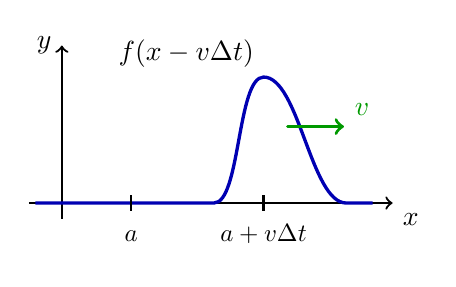
\begin{tikzpicture}
	  \draw[->,thick] (-0.1*\xmax,0) -- (\xmax,0) node[below right] {$x$};
	  \draw[->,thick] (0,-0.1*\ymax) -- (0,\ymax) node[left] {$y$};
	  \wave{0.4}
	  \node[above left] at (F) {$f(x-v\Delta t)$};
	  %\node[left] at (1*\xmax,0.9*\ymax) {$t=\Delta t$};
	  \tick{\xpeak{0.0},0}{90} node[scale=0.9,below] {\strut$a$};
	  \tick{\xpeak{0.4},0}{90} node[scale=0.9,below] {\strut$a+v\Delta t$};
	  \draw[vvec] (F)++(-64:0.35*\ymax) --++ (\v,0) node[above right] {$v$};
	\end{tikzpicture}	
	}
	\only<2>{
		\includegraphics[scale=0.5]{ECE343/longitudinal_waves}
	}
	\end{textblock}
		
\end{frame}

%%%%%%%%%%%%%%%%%%%%%%%%%%%%%%%%%%%%%%%%%%%%%%%%%%%%%
%%%%%%%%%%%%%%%%%%%%%%%%%%%%%%%%%%%%%%%%%%%%%%%%%%%%%

\begin{frame}{Wave Animation}
\begin{textblock}{14.5}(0.5,3)

\href{\mygraphicspath/ECE343/decaying_wave.gif}{\includegraphics[scale=0.6]{\mygraphicspath/ECE343/decaying_wave_init.png}}

\end{textblock}

\end{frame}


%%%%%%%%%%%%%%%%%%%%%%%%%%%%%%%%%%%%%%%%%%%%%%%%%%%%%
%%%%%%%%%%%%%%%%%%%%%%%%%%%%%%%%%%%%%%%%%%%%%%%%%%%%%
\section{Math Review}
\begin{frame}{Remember Euler?}

\begin{textblock}{14.5}(0.5,4)
	$ e^{j\theta} = $ \handoutgap{2in}{$\cosp{\theta} + j\sinp{\theta}$}
	
	\vspace{1cm}
	
	$ e^{-j\theta} = $ \handoutgap{2in}{$\cosp{\theta} - j\sinp{\theta}$}
	
	\vspace{1cm}
	
	$ \cosp{\omega t} = $ \handoutgap{2in}{$\dfrac{e^{j\omega t} + e^{-j\omega t} }{2}$}
	
	\vspace{1cm}
	
	$ \sinp{\omega t} = $ \handoutgap{2in}{$\dfrac{e^{j\omega t} - e^{-j\omega t} }{j2}$}
\end{textblock}

\end{frame}

%%%%%%%%%%%%%%%%%%%%%%%%%%%%%%%%%%%%%%%%%%%%%%%%%%%%%
%%%%%%%%%%%%%%%%%%%%%%%%%%%%%%%%%%%%%%%%%%%%%%%%%%%%%

\begin{frame}{Phasors}
\begin{textblock}{14.5}(0.5,3)
%	\includegraphics[scale=0.4]{./figures/phasors_final}
	\input{\mygraphicspath/ECE343/phasors}
\end{textblock}

\end{frame}


